\subsection{Subpaso 2-A: Ingresar datos del usuario}
Para poder registrar a un usuario nuevo se tienen que ingresar los siguientes datos en la interfaz
\begin{figure}[hbtp]
		
		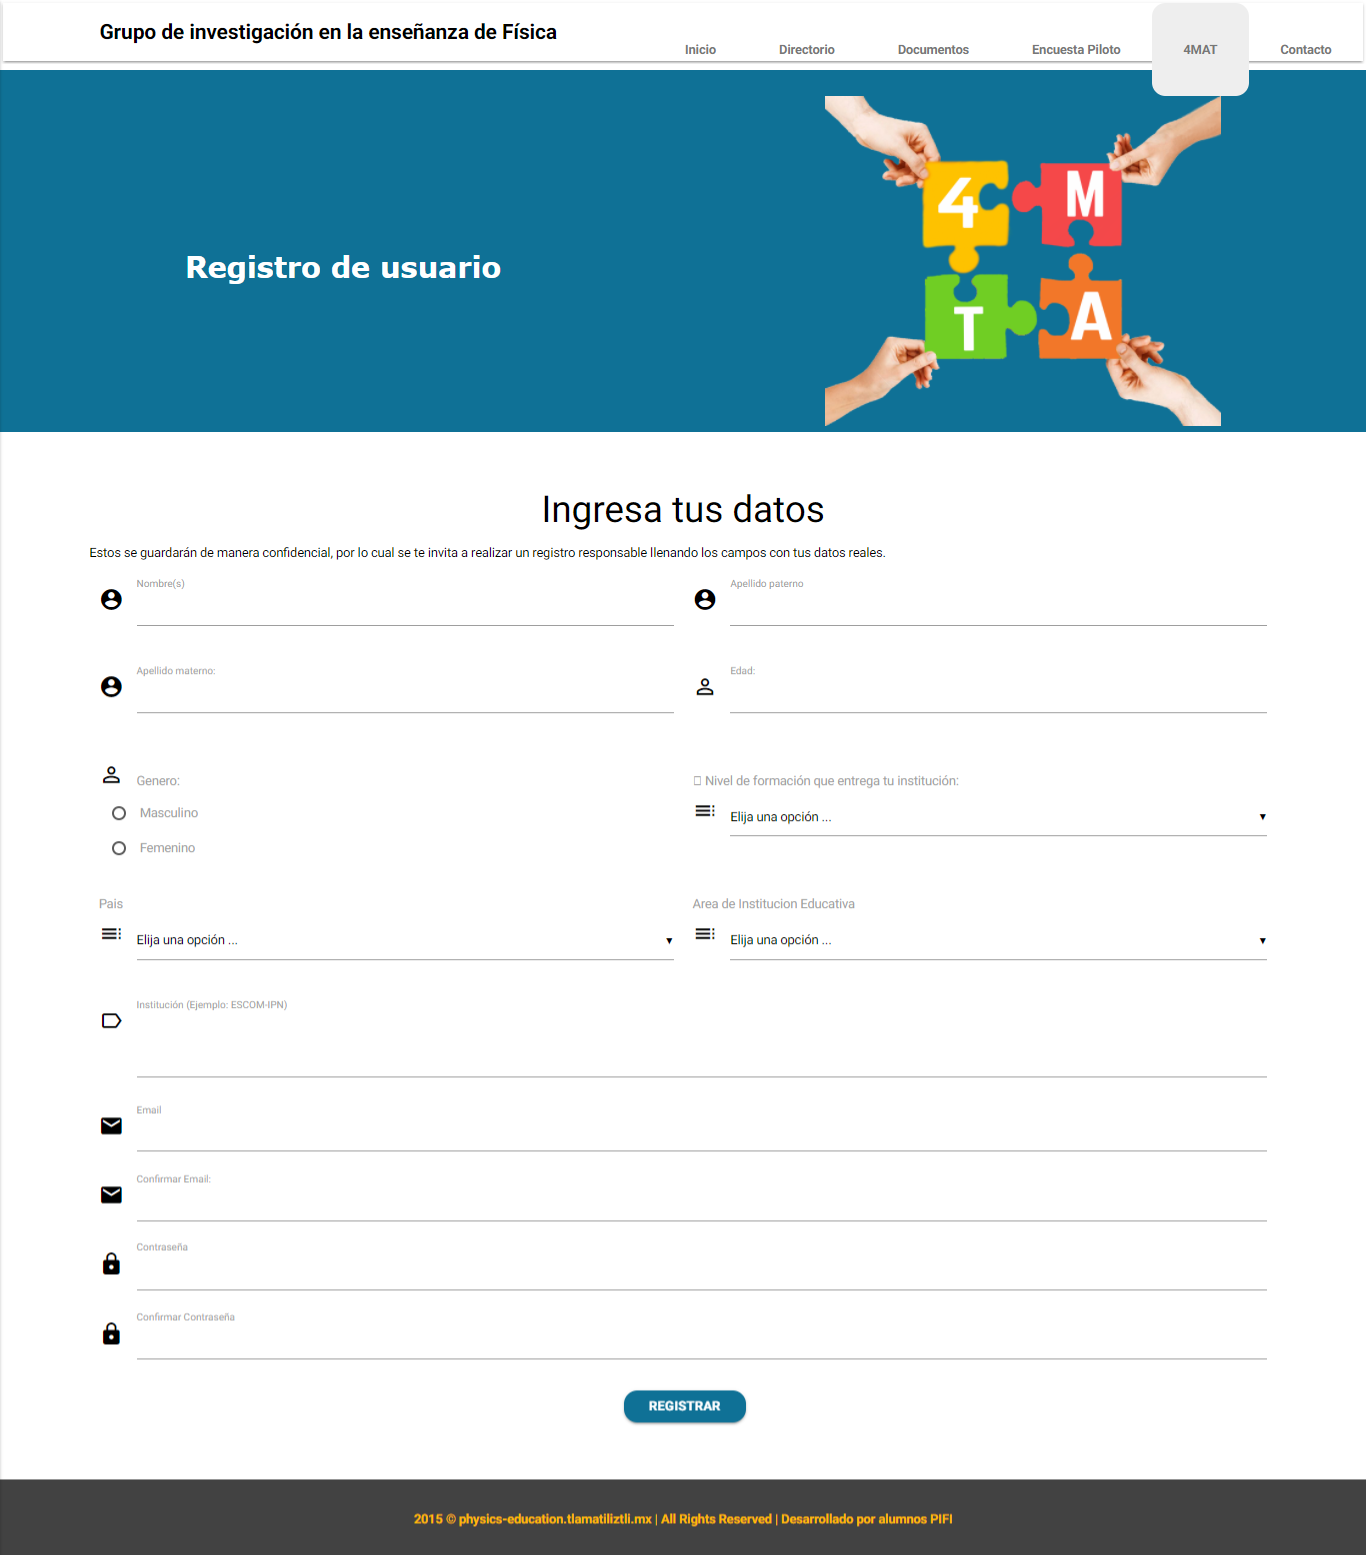
\includegraphics[scale=0.3]{images/Interfaz/IUGS11_registrarUsusario.png}
		\caption{Registro}
	\end{figure}
\begin{enumerate}

	\item Ingrese el nombre completo del usuario.
	\item Ingrese la edad del usuario en números. 
	\item Seleccione el genero del usuario. 
	\begin{itemize}
		\item Masculino
		\item Femenino
	\end{itemize}
	\item Ingrese el nivel de formación que entrega la institución.
		\begin{itemize}
			\item Secundaria
			\item Bachillerato o preparatoria.
			\item Universidad
			\item Posgrado
		\end{itemize}
	\item Ingrese el área de Institución Administrativa.
		\begin{itemize}
			\item Ciencias Físico Matemáticas 
			\item Ciencias Medico Biológicas 
			\item Ciencias Sociales y Administrativas.
		\end{itemize}
	\item Ingrese la Institución del usuario. 
	
	
	\item Ingresa el correo electrónico del usuario.
	\item Ingresa el correo nuevamente para su verificación
	
	\item Ingrese una contraseña 
	\item Repita la contraseña nuevamente para u verificación.
	
	\item presiona el botón \textbf{Registrar}.
	\item En la pantalla nos mostrara un mensaje de \textbf{Usuario registrado exitosamente} en caso de ningun error, de lo contrario mostrará donde hubo un error.
\end{enumerate}

	